\subsection{Preprocessing}
In this subsection, we discuss the preprocessing methods used in our machine learning pipeline.
We cover the following normalization techniques: Z-Score standardization, Max Absolute scaling, Min-Max normalization, robust scaling, Norm 3, power transformation, and quantile transformation.
These techniques are essential for standardizing data, handling different scales, and improving the performance of machine learning models.
For the purposes of this discussion, let $\mathbf{x}$ be a feature vector with values $x_1, x_2, \ldots, x_n$.

\subsubsection{Z-Score Standardization}
Z-Score Standardization, also known as zero-mean normalization, transforms data to have a mean of zero and a standard deviation of one.
This technique is useful when the actual minimum and maximum of a feature are unknown or when outliers may significantly skew the distribution.
The Z-Score Standardization of a feature vector \(\mathbf{x}\) is given by:

$$
x'_i = \frac{x_i - \overline{\mathbf{x}}}{\sigma_\mathbf{x}},
$$

where \(x_i\) is the original value, \(\overline{\mathbf{x}}\) is the mean of the feature vector \(\mathbf{x}\), \(\sigma_\mathbf{x}\) is the standard deviation of the feature vector \(\mathbf{x}\), and \(x'_i\) is the normalized feature value.
By transforming the data using the Z-score, each value reflects its distance from the mean in terms of standard deviations.
Z-Score Standardization is particularly advantageous in scenarios where data features have different units or scales, or when preparing data for algorithms that assume normally distributed inputs~\cite{dataminingConcepts}.

\subsubsection{Max Absolute Scaler}
Max absolute scaling is a normalization technique that scales each feature individually so that the maximum absolute value of each feature is 1.
This results in the data being normalized to a range between -1 and 1.
The formula for max absolute scaling is given by:
$$
	X_{\text{scaled}} = \frac{x}{\max(|x|)},
$$
where $x$ is the original feature value and $X_{\text{scaled}}$ is the normalized feature value.
This scaling method is useful for data that has been centered at zero or data that is sparse, as max absolute scaling does not center the data.
This maintains the sparsity of the data by not introducing non-zero values in the zero entries of the data~\cite{Vasques2024}.
\subsubsection{Min-Max Normalization}\label{subsec:min-max}
Min-Max normalization rescales the range of features to a specific range $[a, b]$, where $a$ and $b$ represent the new minimum and maximum values, respectively.
The goal is to normalize the range of the data to a specific scale, typically 0 to 1.
The Min-Max normalization of a feature vector $\mathbf{x}$ is given by:

$$
x'_i = \frac{x_i - \min(\mathbf{x})}{\max(\mathbf{x}) - \min(\mathbf{x})}(b - a) + a,
$$

where $x_i$ is the original value, $\min(\mathbf{x})$ and $\max(\mathbf{x})$ are the minimum and maximum values of the feature vector $\mathbf{x}$, respectively, and $x'_i$ is the normalized feature value.

This type of normalization is beneficial because it ensures that each feature contributes equally to the analysis, regardless of its original scale~\cite{dataminingConcepts}.
\subsubsection{Robust Scaler}
The robust scaler is a normalization technique that removes the median and scales the data according to the quantile range.
The robust scaler of a feature vector $\mathbf{x}$ is given by:

$$
x'_i = \frac{x_i - \text{Q1}(\mathbf{x})}{\text{Q3}(\mathbf{x}) - \text{Q1}(\mathbf{x})} \: ,
$$

where $x_i$ is the original feature value, $\text{Q1}(\mathbf{x})$ is the first quartile of the feature vector $\mathbf{x}$, and $\text{Q3}(\mathbf{x})$ is the third quartile of the feature vector $\mathbf{x}$.
This technique can be advantageous in cases where the data contains outliers, as it relies on the median and quantile range instead of the mean and variance, both of which are sensitive to outliers~\cite{Vasques2024}.
\subsubsection{Norm 3}
As previously mentioned, the \gls{chemcam} instrument consists of three spectrometers, each producing 2048 channels.
For data normalization, we follow the approach taken by the ChemCam team and normalize across individual spectrometers' wavelength ranges, a process known as \textit{Norm 3}~\cite{cleggRecalibrationMarsScience2017, andersonImprovedAccuracyQuantitative2017}.
This method ensures that the wavelength intensities captured by each spectrometer are normalized independently, thus preserving the relative intensities within each spectrometer.

Figure~\ref{fig:spectral_plot} shows a spectral plot of the \gls{ccs} data for the \textit{ultramafic} sample, illustrating the three distinct spectral regions, each captured by one of the three spectrometers.
Specifically, one spectrometer captures the \gls{uv} region, another captures the \gls{vio} region, and the third captures the \gls{vnir} region.

\begin{figure}[H]
	\centering
	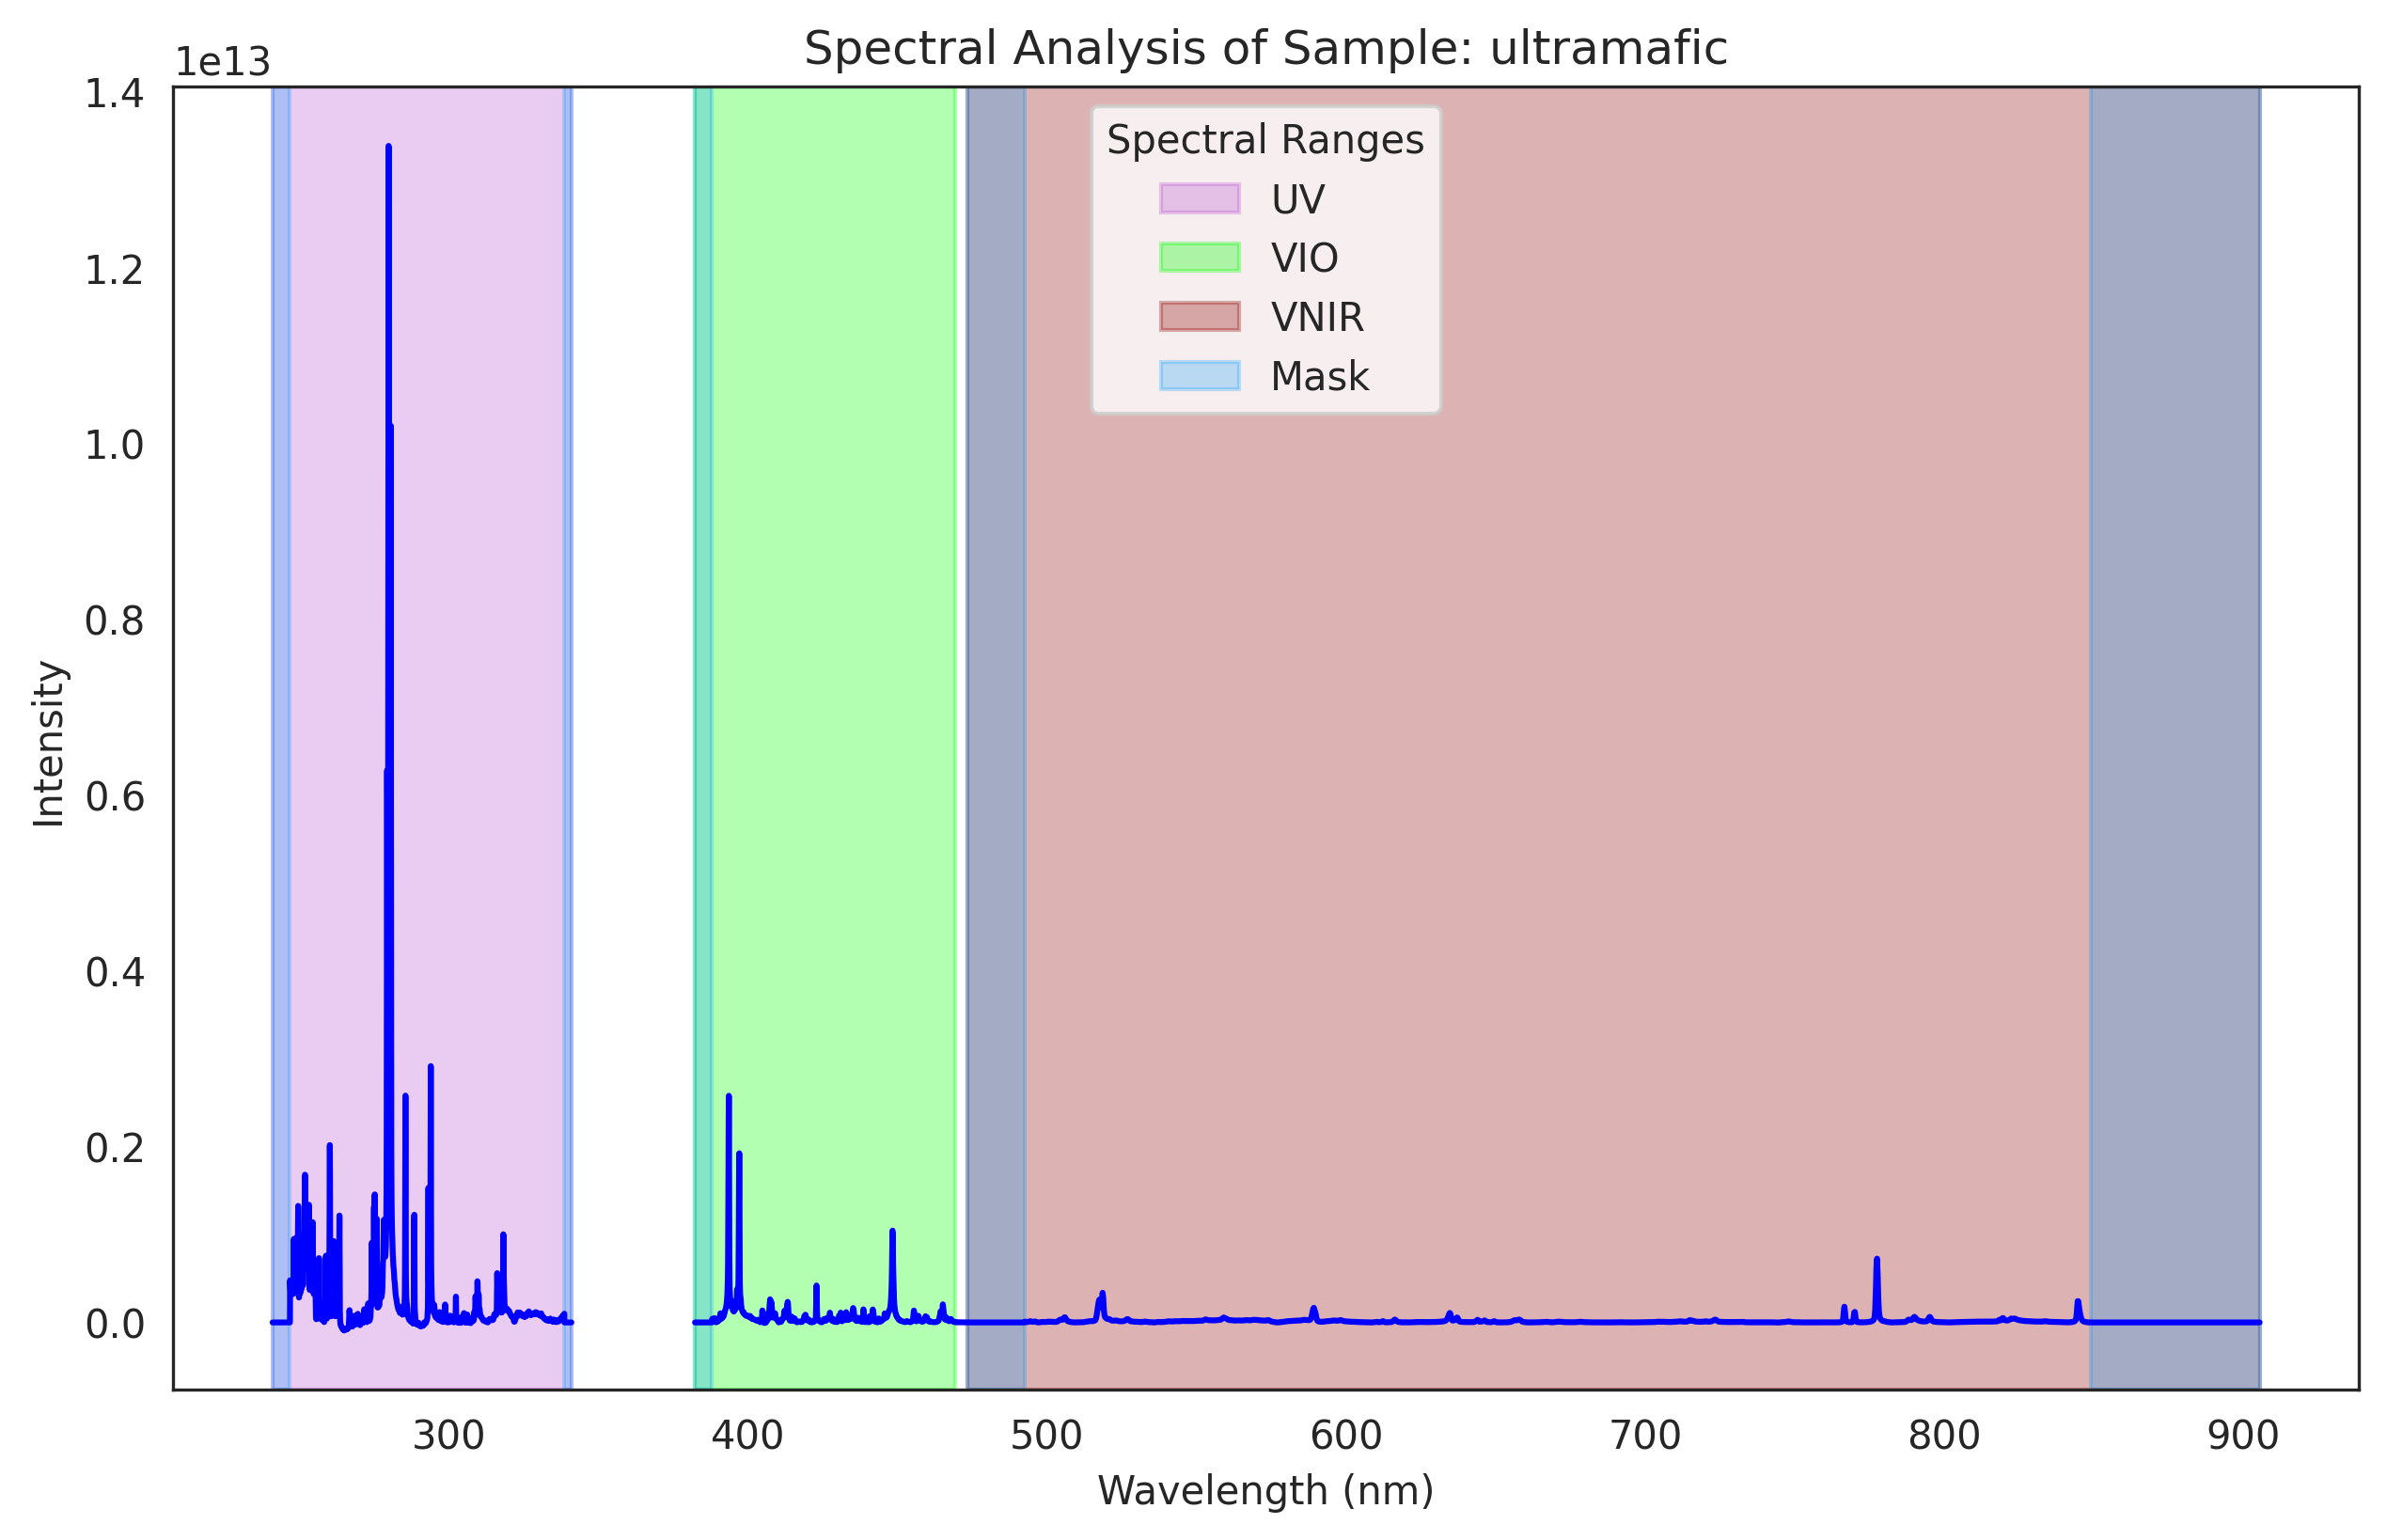
\includegraphics[width=0.5\textwidth]{images/spectral_plot.png}
	\caption{Spectral plot of the \gls{ccs} data for the \textit{ultramafic} sample. The wavelengths represent the spectral channels.}
	\label{fig:spectral_plot}
\end{figure}

Let $\gamma$ represent the spectrometer index, where $\gamma \in \{1, 2, 3\}$, corresponding to the \gls{uv}, \gls{vio}, and \gls{vnir} spectrometers, respectively.
Then, Norm 3 is formally defined as:

\begin{equation}
	\tilde{X}_{i,j}^{(\gamma)} = \frac{X_{i,j}^{(\gamma)}}{\sum_{j=1}^{N} X_{i,j}^{(\gamma)}},
\end{equation}

where

\begin{itemize}
	\item $\tilde{X}_{i,j}^{(\gamma)}$ is the normalized wavelength intensity for the $i$-th sample in the $j$-th channel on the $\gamma$-th spectrometer,
	\item $X_{i,j}^{(\gamma)}$ is the original wavelength intensity for the $i$-th sample in the $j$-th channel on the $\gamma$-th spectrometer, and
	\item $N = 2048$ is the number of channels in each spectrometer.
\end{itemize}

This normalization method results in a total of $3N = 6144$ normalized features for each sample, as each of the three spectrometers contributes 2048 channels.
\subsubsection{Power Transformation}
Power transformations are a class of mathematical functions used to stabilize variance and make data more closely approximate a normal distribution.
They are particularly useful in statistical modeling and data analysis to meet the assumptions of linear models.

One of the first influential power transformation techniques is the Box-Cox power transform, introduced by \citet{BoxAndCox} in 1964.
This is defined for positive data and is aimed at normalizing data or making it more symmetric.
For a feature vector $\mathbf{x}$, the Box-Cox transformation is defined as:

$$
\psi^{\text{BC}}(\lambda, \mathbf{x}) =
\begin{cases}
\frac{\mathbf{x}^\lambda - 1}{\lambda}, & (\lambda \neq 0) \\
\log(\mathbf{x}), & (\lambda = 0)
\end{cases},
$$

where $\lambda$ is the transformation parameter.
$\lambda$ determines the extent and nature of the transformation, where positive values of $\lambda$ apply a power transformation and $\lambda = 0$ applies a logarithmic transformation.

To overcome the limitations of the Box-Cox transformation, \citet{YeoJohnson} introduced a new family of power transformations that can handle both positive and negative values.
The Yeo-Johnson power transformation is defined as:

$$
\psi(\lambda, \mathbf{x}) =
\begin{cases}
\frac{(\mathbf{x} + 1)^\lambda - 1}{\lambda} & (\mathbf{x} \geq 0, \lambda \neq 0) \\
\log(\mathbf{x} + 1) & (\mathbf{x} \geq 0, \lambda = 0) \\
- \frac{(-\mathbf{x} + 1)^{2 - \lambda} - 1}{2 - \lambda} & (\mathbf{x} < 0, \lambda \neq 2) \\
-\log(-\mathbf{x} + 1) & (\mathbf{x} < 0, \lambda = 2)
\end{cases}
$$

For non-negative values, the Yeo-Johnson transformation simplifies to the Box-Cox transformation, making them equivalent in this context.
The key benefit of the Yeo-Johnson transformation is its ability to handle any real number, making it a robust choice for transforming data to achieve approximate normality or symmetry.
This property is particularly beneficial for preparing data for statistical analyses and machine learning models that require normally distributed input data.
\subsubsection{Quantile Transformer}
Quantile transformation is a method that applies a non-linear transformation to map data to a uniform or normal distribution.
This process involves mapping the data $X$ to a set of probabilities $p$ using the \gls{cdf}, which indicates the probability that a random variable will be less than or equal to a specific value in $X$'s original distribution.
Subsequently, the quantile function, which is the inverse of the \gls{cdf} of the desired distribution, is applied to these probabilities $p$ to generate the transformed data.
This method forces the data to conform to the specified distribution regardless of the original distribution's form~\cite{Vasques2024}.
\subsubsection{Principal Component Analysis (PCA)}\label{subsec:pca}
\gls{pca} is a dimensionality reduction technique used to reduce the number of features in a dataset while retaining as much information as possible.
We provide an intuitive explanation of \gls{pca} in this section based on \citet{dataminingConcepts} and \citet{Vasques2024}.

\gls{pca} works by identifying the directions in which the\\$n$-dimensional data varies the most and projects the data onto these $k$ dimensions, where $k \leq n$.
This projection results in a lower-dimensional representation of the data.
\gls{pca} can reveal the underlying structure of the data, which enables interpretation that would not be possible with the original high-dimensional data.

\gls{pca} works as follows.
First, the input data are normalized, which prevents features with larger scales from dominating the analysis.

Then, the covariance matrix of the normalized data is computed.
The covariance matrix captures how each pair of features in the dataset varies together.
$k$ orthogonal unit vectors, called \textit{principal components}, are then computed from this covariance matrix.
These vectors are perpendicular to each other and capture the directions of maximum variance in the data.

The principal components are then sorted such that the first component captures the most variance, the second component captures the second most variance, and so on.
Variance is assumed by \gls{pca} to be a measure of information.
In other words, the principal components are sorted based on the amount of information they capture.

After computing and sorting the principal components, the data can be projected onto the most informative principal components.
This projection results in a lower-dimensional approximation of the original data.
The number of principal components to keep is a hyperparameter that can be tuned to balance the trade-off between the amount of information retained and the dimensionality of the data.

\subsubsection{Kernel PCA}
We provide a brief overview of the \gls{kernel-pca} algorithm based on \citet{learningwithkernels}.
\gls{kernel-pca} is an extension of traditional \gls{pca} designed to handle nonlinear relationships among data points.
The core idea behind \gls{kernel-pca} is to map data into a higher-dimensional space using a kernel function, a technique known as the kernel trick.
This mapping enables linear separation of data points in the higher-dimensional space, even if they are not linearly separable in the original space.

Similar to \gls{pca}, as described in Section~\ref{subsec:pca}, the goal of \gls{kernel-pca} is to extract the principal components of the data.
Unlike \gls{pca}, \gls{kernel-pca} does not compute the covariance matrix of the data directly, as this is often infeasible for high\\-dimensional datasets.
Instead, \gls{kernel-pca} leverages the kernel trick to compute the similarities between data points directly in the original space using a kernel function.
This kernel function implicitly computes the dot product in the higher-dimensional feature space without explicitly mapping the data points into that space.
That way, \gls{kernel-pca} can capture nonlinear relationships among data points without explicitly transforming them into a higher-dimensional space.

By using pairwise similarities to construct a kernel matrix, also referred to as a Gram matrix, \gls{kernel-pca} can perform eigenvalue decomposition.
This process allows for the extraction of principal components in the feature space, similar to the approach used in regular \gls{pca}.
However, in \gls{kernel-pca}, the eigenvalue decomposition is performed on the kernel matrix rather than the covariance matrix, allowing for the extraction of nonlinear principal components.